%!TEX root=paper/thesis.tex
\section{Method}\label{sec:clf_method}

\PM{MDP}
We model the \textbf{feature selection} policy $\pi(x): \mathcal{X} \mapsto 2^\mathcal{A}$ following the reinforcement learning approach as described in \autoref{sec:mdp_formulation}.
The set of \textbf{actions} $\mathcal{A}$ is exactly the set of features $\mathcal{H}$.
The policy learning approach remains the same, including implementation details.
Three things are different: the reward definition, the state featurization function, and the additional dependence on a classifier.

\PM{Classifier}
We defer discussion of learning the \textbf{feature combination} classifier $g(\mathcal{H}_\pi) : 2^\mathcal{H} \mapsto \mathcal{Y}$ to~\autoref{sec:clf_classifier}.
For now, we assume that $g$ can combine an arbitrary subset of features and provide a distribution $P(Y = y)$.
For example, $g$ could be a Naive Bayes (NB) model trained on the fully-observed data.

%!TEX root=paper/thesis.tex
\subsection{Reward definition}\label{sec:clf_reward}

\begin{figure}[ht]
\centering
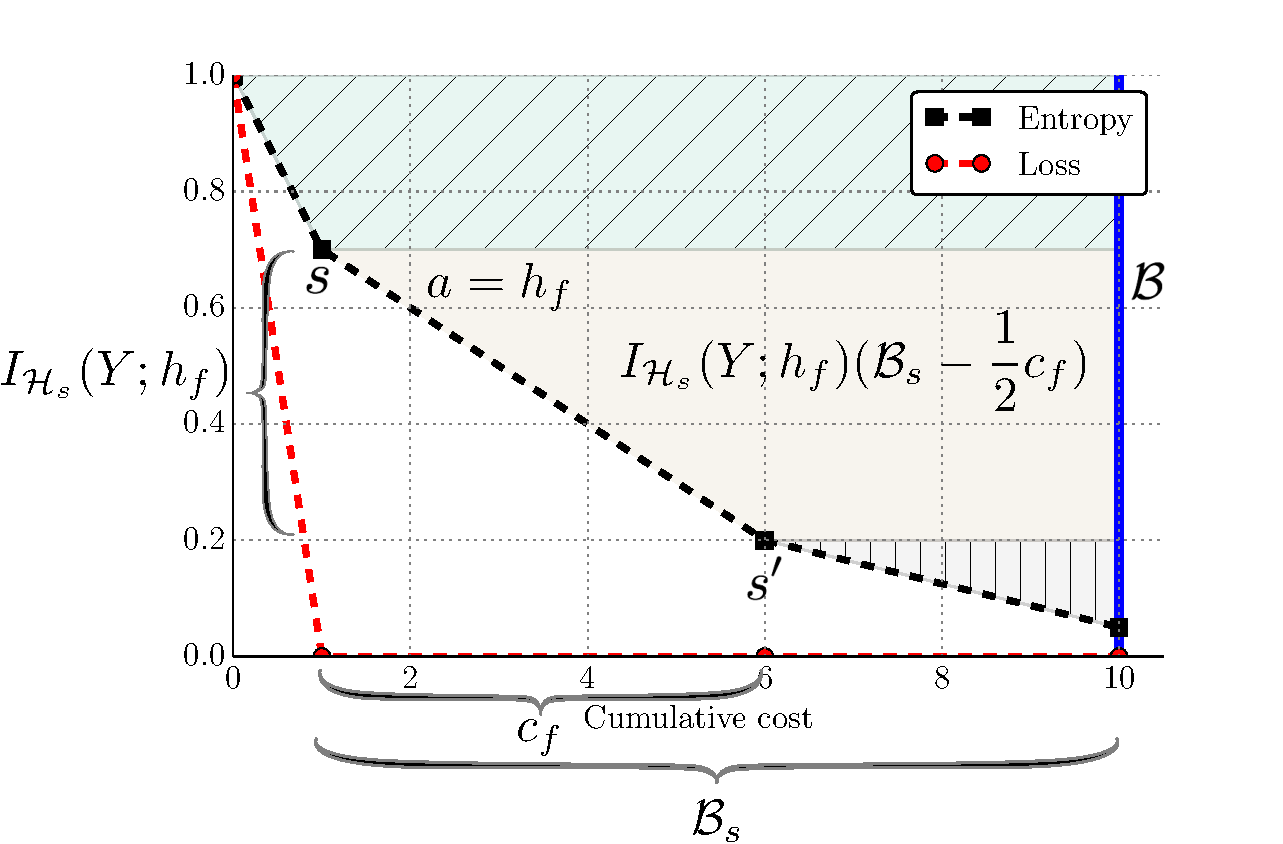
\includegraphics[width=.8\linewidth]{../../figures/rewards.pdf}
\caption{
Definition of the reward function.
To maximize the total area above the entropy vs. cost curve from $0$ to $\mathcal{B}$, we define the reward of an individual action as the area of the slice of the total area that it contributes.
From state $s$, action $a = h_f$ leads to state $s'$ with cost $c_f$.
The information gain is $I_{\mathcal{H}_s}(Y; h_f) = H(Y; \mathcal{H}_s) - H(Y; \mathcal{H}_s \cup {h_f})$.
\label{fig:clf_rewards}}
\end{figure}


\PM{Loss vs. cost}
The budget-sensitive loss $\mathcal{L}_\mathcal{B}$ enforces Anytime performance by valuing early gains more than later gains.
To formalize this, consider \hyperref[fig:clf_rewards]{Figure~\ref*{fig:clf_rewards}}, which shows the entropy and the 0-1 loss of $g$ at every point in a sequential feature selection episode for some instance $x$.
For the best Anytime performance, we want to capture the most area above the loss vs. cost curve, up to max budget $\mathcal{B}$ \parencite{Karayev-NIPS-2012}.
Recall from \eqref{eq:expected_reward} that the value of an episode $\xi$ is defined as the sum of obtained rewards.
If the reward of a single action is defined as the area above the curve that is captured as a direct result, then the value of the whole episode exactly corresponds to $\mathcal{L}_\mathcal{B}$.

\PM{Infogain}
However, there is a problem with using loss directly: only the first action to ``tip the scale'' toward the correct prediction gets a direct reward (in the figure, it is the first action).
A smoother reward function is desirable: if the classifier $g$ can give a full distribution $P(Y = y \mid \mathcal{H}_{\pi(x)})$ and not just a prediction $\hat{y} \in \mathcal{Y}$, we can maximize the \emph{information gain} of the selected subset instead of directly minimizing the loss of $g(\pi(x))$:
\begin{eqnarray}
I(Y; \mathcal{H}_{\pi(x)}) &=& H(Y) - H(Y | \mathcal{H}_{\pi(x)}) = \\ \notag
&=& \sum_{y \in Y} P(y) \log P(y) - \\ \notag
&&\sum_{y, \mathcal{H}_{\pi(x)}} P(y, \mathcal{H}_{\pi(x)}) \log P(y \mid \mathcal{H}_{\pi(x)})
\end{eqnarray}

\PM{Definition}
To the extent that $g$ is unbiased, maximizing information gain corresponds to minimizing loss, and ensures that we not only make the right classification decision but also become maximally certain.
Therefore, as graphically presented in \hyperref[fig:clf_rewards]{Figure~\ref*{fig:clf_rewards}}, we define the reward of selecting feature $h_s$ with cost $c_f$ with the set $\mathcal{H}_s$ computed to be $I_{\mathcal{H}_s}(Y; h_f) (\mathcal{B}_s - \frac{1}{2}c_f)$.
Although we do not evaluate in this regime, note that this definition easily incorporates a \textbf{setup cost} in addition to \textbf{deadline cost} by only computing the area in between setup and deadline costs.


%!TEX root=paper/paper.tex
\subsection{Features of the state}\label{sec:clf_features}

The featurization function $\phi(s)$ extracts the following features from the state:

\begin{itemize}\addtolength{\itemsep}{-.5\baselineskip}
\item Bit vector $\textbf{m}$ of length $F$: initially all bits are $1$ and are set to $0$ when the corresponding feature is computed.
\item For each $h_f$, a vector of size $d_f$ representing the values; $0$ until observed.
\item Cost feature $c \in [0, 1]$, for fraction of the budget spent.
\item Bias feature $1$.
\end{itemize}

\PM{Static vs Dynamic}
These features define the \textbf{dynamic} state, presenting enough information to have a \emph{closed-loop} (dynamic) policy that may select different features for different test instances.
The \textbf{static} state has all of the above features except for the observed feature values.
This enables only an \emph{open-loop} (static) policy, which is exactly the same for all instances.
Policy learned with the static state is used as a baseline in experiments.


\subsection{Learning the classifier.}\label{sec:classifier}

We have so far assumed that $g$ can combine an arbitrary subset of features and provide a distribution $P(Y = y)$---for example, a Gaussian Naive Bayes (NB) model trained on the fully-observed data.
However, a Naive Bayes classifier suffers from its restrictive independence assumptions.

Since discriminative classifiers commonly provide better performance, we use a \textbf{logistic regression} classifier, which presents a new challenge: at test time, some feature values are missing and need to be imputed.

If the classifier is trained exclusively on fully-observed data, then the feature value statistics at test time will not match, resulting in poor performance.
Therefore, we need to learn classifier weights on a distribution of data that exhibits the pattern of missing features induces by the policy $\pi$.
At the same time, learning the policy depends on the classifier $g$, used in the computation of the rewards.

\begin{algorithm}[]
\SetKwFunction{ComputeRewards}{ComputeRewards}
\SetKwFunction{GatherSamples}{GatherSamples}
\SetKwFunction{UpdatePolicy}{UpdatePolicy}
\SetKwFunction{UpdateClassifier}{UpdateClassifier}

\SetAlgoLined
\KwIn{$\mathcal{D} = \{x_n, y_n\}_{n=1}^N$; $\mathcal{L}_\mathcal{B}$}
\KwResult{Trained $\pi$, $g$}
\BlankLine
$\pi_0 \leftarrow$ random\;
\For {$i \leftarrow 1$ \KwTo max\_iterations} {
    States, Actions, Costs, Labels $\leftarrow$ \GatherSamples{$\mathcal{D}$, $\pi_{i-1}$}\;
    $g_i \leftarrow$ \UpdateClassifier{States, Labels}\;
    Rewards $\leftarrow$ \ComputeRewards{States, Costs, Labels, $g_i, \mathcal{L}_\mathcal{B}, \gamma$}\;
    $\pi_i \leftarrow$ \UpdatePolicy{States, Actions, Rewards}\;
}
\caption{Because reward computation depends on the classifier, and the distribution of states depends on the policy, $g$ and $\pi$ are trained iteratively.\label{alg:learning}}
\end{algorithm}


For this reason, the policy and classifier need to be learned jointly: \autoref{alg:learning} gives the iterative procedure.
In summary, we start from random $\pi$ and $g$, gather a batch of trajectories.
The batch is used to update both $g$ and $\pi$.
Then new trajectories are generated with the updated $\pi$, rewards are computed using the updated $g$, and the process is repeated.
This is a variant of generalized policy iteration \cite{Sutton1998}.

\paragraph{Unobserved value imputation.}
Unlike the Naive Bayes classifier, the logistic regression classifier is not able to use an arbitrary subset of features $\mathcal{H}_\pi$, but instead operates on feature vectors of a fixed size.
To represent the feature vector of a fully observed instance, we write $\mathbf{x} = [h_1(x), \dots, h_f(x)]$.
In case that $\mathcal{H}_\pi \subset \mathcal{H}$, we need to fill in unobserved feature values in the vector.

A basic strategy is \textbf{mean imputation}: filling in with the mean value of the feature:
\begin{align}
\mathbf{x}_\pi = \left[ h_i(x) : \left\{ \begin{array}{rl}
 h_i(x) &\mbox{ if $h_i \in \mathcal{H}_{\pi(x)}$} \\
 \bar{\mathbf{h}}_i &\mbox{ otherwise}
\end{array} \right. \right]
\end{align}

If we assume that $\mathbf{x}$ is distributed according to a multivariate Gaussian $\mathbf{x} \sim \mathcal{N}(\mathbf{0}, \Sigma)$, where $\Sigma$ is the sample covariance $X^T X$ and the data is standardized to have zero mean, then it is possible to do \textbf{Gaussian imputation}.
Given a feature subset $\mathcal{H}_\pi$, we write:
\begin{equation}
\mathbf{x}_\pi = \begin{bmatrix} \mathbf{x}^\text{o}\\  \mathbf{x}^\text{u} \end{bmatrix} \sim \mathcal{N} \left( \mathbf{0}, \begin{bmatrix} \mathbf{A} & \mathbf{C}\\ \mathbf{C}^T & \mathbf{B} \end{bmatrix} \right)
\end{equation}
where $\mathbf{x}^\text{o}$ and $\mathbf{x}^\text{u}$ represent the respectively observed and unobserved parts of the full feature vector $\mathbf{x}$.
%, $\mathbf{A}$ is the covariance matrix of $\mathbf{x}^\text{o}$, $\mathbf{B}$ is the covariance matrix of $\mathbf{x}^\text{u}$, and $C$ is the cross-variance matrix that has as many rows as the size of $\mathbf{x}^\text{o}$ and as many columns as the size of $\mathbf{x}^\text{u}$.
%\parencite{Roweis-gaussian-identities}.
In this case, the distribution over unobserved variables conditioned on the observed variables is given as
$\mathbf{x}^\text{u} \mid \mathbf{x}^\text{o} \sim \mathcal{N} \left( \mathbf{C}^T \mathbf{A}^{-1} \mathbf{x}^\text{o},\, \mathbf{B} - \mathbf{C}^T \mathbf{A}^{-1} \mathbf{C} \right)$.

\paragraph{Learning more than one classifier.}
As illustrated in \hyperref[fig:state_space]{Figure~\ref*{fig:state_space}}, the policy $\pi$ selects some feature subsets more frequently than others.
Instead of learning only one classifier $g$ that must be robust to all observed feature subsets, we can learn several classifiers, one for each of the most frequent subsets.
This is done by maintaining a distribution over encountered feature subsets during training.
For each of the $K$ most frequent subsets, a separate classifier is trained, using data that is closest by Hamming distance on the selected-feature bit vector.

Each classifier is trained with the \textsc{Liblinear} implementation of logistic regression, with $L_2$ regularization parameter K-fold cross-validated at each iteration.

\begin{figure}[ht]
\centering
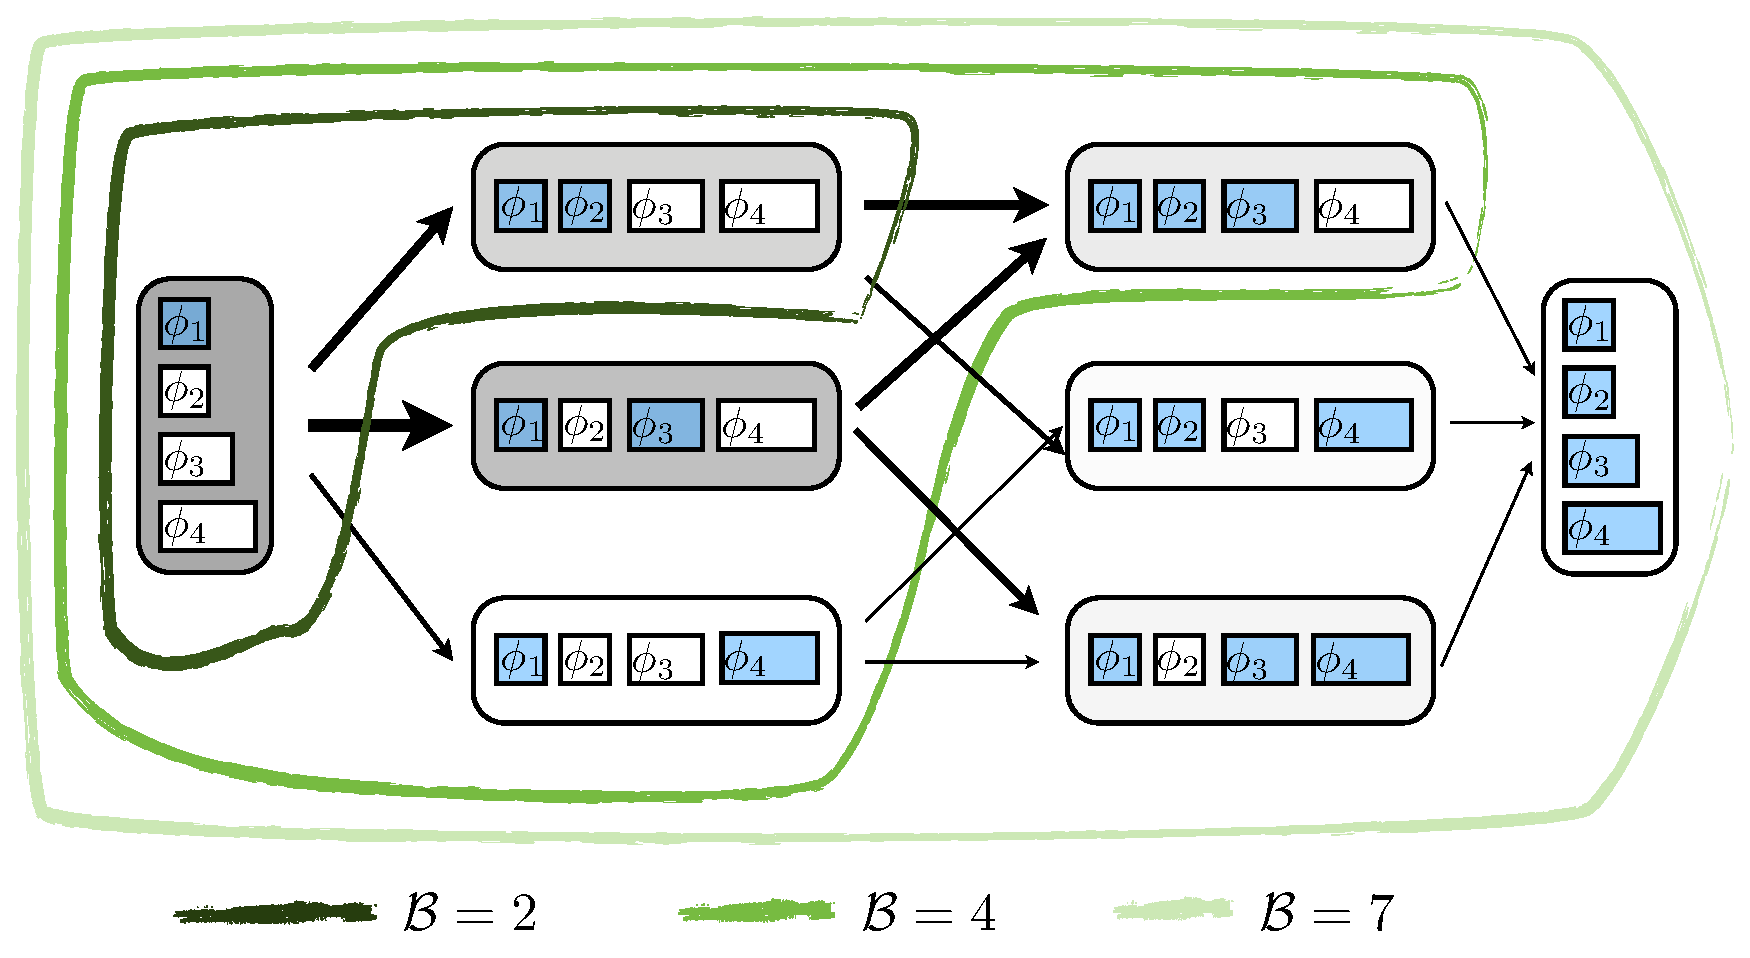
\includegraphics[width=1\linewidth]{../../figures/mdp_masks.pdf}
\caption{
The action space $\mathcal{A}$ of the MDP is the the set of features $\mathcal{H}$, represented by the $\phi$ boxes.
The primary discretization of the state space can be visualized by the possible feature subsets (larger boxes); selected features are colored in the diagram.
The feature selection policy $\pi$ induces a distribution over feature subsets, for a dataset, which is represented by the shading of the larger boxes.
Not all states are reachable for a given budget $\mathcal{B}$.
In the figure, we show three ``budget cuts'' of the state space.
\label{fig:state_space}
}
\end{figure}

